\section{Fichiers et repertoires}
\subsection{Les noms et contenus des fichiers}
\begin{frame}{Noms et contenu des fichiers}
  \begin{block}{La décomposition traditionnelle d'un nom de fichier}
    \begin{columns}
      \begin{column}{8cm}
        Deux parties séparées par un point:
        \begin{itemize}
        \item La $1\up{ère}$ partie informe sur la nature du contenu du
          fichier,
        \item La $2\up{ème}$ partie informe sur le format ou la finalité des données.
        \end{itemize}
      \end{column}
      \begin{column}{3cm}
        \begin{tabular}{|r@{}r@{}l|}
          \hline
          {\color{solarizedRed}nom}&.&{\color{solarizedGreen}extension} \\
          {\color{solarizedRed}prefix}&.&{\color{solarizedGreen}suffix} \\
          {\color{solarizedRed}description}&.&{\color{solarizedGreen}format}\\
          \hline
        \end{tabular}
      \end{column}
    \end{columns}
  \end{block}
  \begin{columns}
    \begin{column}{5.5cm}
      \begin{block}{Exemples de formats de fichiers}
        \begin{center}
          \begin{tabular}{ll}
            \hline
            Extension&Contenu\\
            \hline
            .c&Sources C\\
            .html&Document Web\\
            .pdf&Document Mis en page\\
            .txt&Texte brut\\
            .mp3&Fichier Multimedia\\
            \hline
          \end{tabular}
        \end{center}
      \end{block}
    \end{column}
    \begin{column}{5.5cm}
      \begin{block}{Exemples de noms de fichiers}
        \begin{center}
          \begin{tabular}{ll}
            \hline
            Enigmatique&Informatif\\
            \hline
            e3.c&teste\_boucle\_for.c\\
            New.pdf&2011\_IntroSys\_cours\_1.pdf\\
            toto.sh&test\_boucle\_for.sh\\
            \hline
          \end{tabular}
        \end{center}
      \end{block}
      \vrule
    \end{column}
  \end{columns}
  \begin{alertblock}{Le choix des noms des fichiers et répertoires}
    \begin{itemize}
    \item Ils doivent être choisis minutieusement pour être informatifs,
    \item Choisir un nom : réfléchir pour un gain de temps pour
      retrouver le fichier ou le répertoire concerné.
    \end{itemize}
  \end{alertblock}
\end{frame}
\subsection{Organisation des données enregistrées}
\begin{frame}{Organisation des données enregistrées}
  \begin{block}{De très nombreux fichiers et répertoires}
    \begin{columns}
      \begin{column}{.7\linewidth}
        \begin{itemize}
        \item Le nombre de fichiers enregistrés sur un disque dur peut
          aisément dépasser 100.000 fichiers,
        \item Chaque fichier est identifié par un nom,
        \item Les fichiers sont regroupés dans des répertoires et
          sous-répertoires.
        \item Chaque répertoire est identifié par un nom.
        \end{itemize}
      \end{column}%
      \begin{column}{.25\linewidth}
        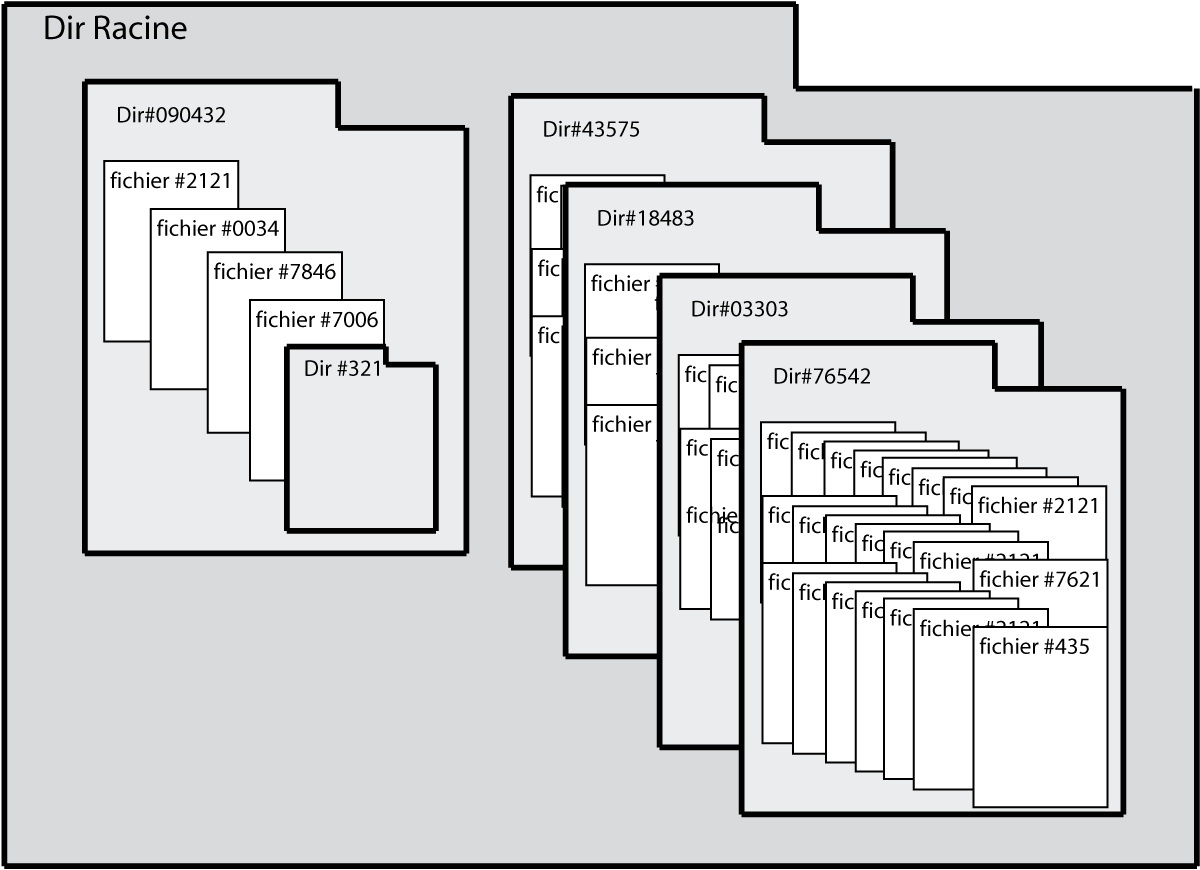
\includegraphics[width=\linewidth]{img/s02/file_system}
      \end{column}
    \end{columns}
  \end{block}
  \begin{block}{Une organisation en arborescence}
    \begin{itemize}
    \item Cette organisation arborescente permet de faciliter la
      recherche d'un fichier,
    \item Les fichiers sont regroupés par application, par thème, par
      format, par fonction, \dots \end{itemize}
  \end{block}
  \begin{alertblock}{Remarque}
    \begin{itemize}
    \item[\dialogerror] Avec tous les fichiers au même
      \textit{endroit}, il est très difficile de les lister (trop à
      lire).
    \item[\dialoginformation] Organisation \emph{hiérarchique} qui permet d'organiser les données et
      de faciliter leur accès.
    \end{itemize}
  \end{alertblock}
\end{frame}

\subsection{L'organisation arborescente}
\begin{frame}{Exemple d'arborescence Linux}
  \dirtree{%
    .1 \DTd{}\DTfcomment{Répertoire Racine ou Root Directory}.  .2
    \DTd{bin}.  .3 (\dots).  .2 \DTd{home}.  .3
    \DTd{chez\_moi}\DTfcomment{Répertoire Personnel ou User
      Directory}.  .4 \DTd{Mes\_Documents}.  .5 ListeDesCourses.txt.
    .5 Exercice\_1.sh.  .4 (\dots).  .3 \DTd{anonymous}.  .4
    LisezMoi.txt.  .4 \DTd{Telechargements}.
    % .5 Cours\_Systeme.pdf.
    .5 (\dots).  .2 (\dots).  }
  \begin{alertblock}{Les répertoires importants}
    \begin{itemize}
    \item La \textbf{racine} (\textit{Root directory}) contient tous
      les répertoires et fichiers accessibles depuis le système.
    \item Le \textbf{répertoire personnel} (\textit{User Directory} ou
      \textit{Home Directory}) est le répertoire dans lequel
      l'utilisateur peut faire ce qu'il veut (écrire, modifier,
      supprimer, installer \dots).
    \end{itemize}
  \end{alertblock}
\end{frame}
\subsection{La notion de Chemin}
\begin{frame}{La notion de Chemin}
  \begin{block}{Le chemin défini un nom unique}
    \begin{itemize}
    \item Deux fichiers ou répertoires ne peuvent pas porter le même nom si ils sont dans un même répertoire.
    \item Les noms des fichiers et répertoires différencient les caractères \textsc{Majuscules} et minuscule. Les fichiers \alert{E}ssai.txt et \alert{e}ssai.txt peuvent donc être dans le même répertoire. 
    \end{itemize}
  \end{block}
  \begin{block}{Exemples de chemins absolus}
    \dirtree{%
      .1 \DTd{}\DTfcomment{Un chemin absolu part de la racine {\color{solarizedAccent}/}}.
      .2 \DTd{home}\DTfcomment{/{\color{solarizedAccent}home/}}.
      .3 \DTd{chez\_moi}\DTfcomment{/home/{\color{solarizedAccent}chez\_moi/}}.
      .4 \DTd{Etoiles}\DTfcomment{/home/chez\_moi/{\color{solarizedAccent}Etoiles/}}.
      .5 SOLEIL.jpg\DTfcomment{/home/chez\_moi/Etoiles/{\color{solarizedAccent}SOLEIL.jpg}}.
      .5 Soleil.jpg\DTfcomment{/home/chez\_moi/Etoiles/{\color{solarizedAccent}Soleil.jpg}}.
      .4 \DTd{Systeme\_Solaire}\DTfcomment{/home/chez\_moi/{\color{solarizedAccent}Systeme\_Solaire/}}.
      .5 SOLEIL.jpg\DTfcomment{/home/chez\_moi/Systeme\_Solaire/{\color{solarizedAccent}SOLEIL.jpg}}.
    }
  \end{block}
  \begin{alertblock}{Syntaxe d'un chemin absolu}
    Le chemin \textit{absolu} d'un fichier ou d'un répertoire est unique. Il donne la liste des répertoires et sous-répertoires en partant de la racine \lin{/} (la référence \textit{absolue} de l'arborescence) jusqu'à la cible.
  \end{alertblock}
\end{frame}

\subsection{Répertoire courant et Chemins relatifs}
\begin{frame}{Répertoire courant et Chemins relatifs}
  \begin{block}{Le répertoire courant}
    \begin{itemize}
    \item Le répertoire courant est un répertoire de référence d'où sont lancées les commandes.
    \item Par défaut, le répertoire courant est le répertoire personnel de l'utilisateur,
    \item Naviguer dans l'arborescence équivaut à modifier le répertoire courant.
    \end{itemize}
  \end{block}
  \begin{block}{Exemples de chemins relatifs}
    \dirtree{%
      .1 \DTd{home}\DTfcomment{../..}.
      .2 \DTd{chez\_moi}\DTfcomment{../}.
      .3 \DTd{Etoiles}\DTfcomment{{\color{solarizedAccent}Répertoire Courant ~~./}}.
      .4 SOLEIL.jpg\DTfcomment{SOLEIL.jpg {\color{black}ou} ./SOLEIL.jpg}.
      .4 Antares.jpg\DTfcomment{Antares.jpg {\color{black}ou} ./Antares.jpg}.
      .3 \DTd{Systeme\_Solaire}\DTfcomment{../Systeme\_Solaire/}.
      .4 terre.gif\DTfcomment{../Systeme\_Solaire/terre.gif}.
    }
  \end{block}
  \begin{alertblock}{Syntaxe d'un Chemin Relatif}
    \begin{itemize}
    \item Le chemin \textit{relatif} d'un fichier ou d'un répertoire donne la liste des répertoires et sous-répertoires en partant du répertoire courant (la référence \textit{relative} dans l'arborescence) jusqu'à la cible.
    \item Il est relatif, car lorsque le répertoire courant change, le chemin relatif change.
    \end{itemize}
  \end{alertblock}
\end{frame}

%%%%%%%%%%%%%% 
\subsection{Notation spéciales}
\begin{frame}{Notation Spéciales}
  \begin{block}{Les chemins des répertoires de référence}
    \begin{columns}
      \begin{column}{6cm}
        \begin{center}
          \begin{tabular}{lr}
            \hline
            Répertoire&Notation\\
            \hline
            Répertoire Racine&\lin{/}\\
            Répertoire Personnel&\lin{\~{}}\\
            \hline
          \end{tabular}
        \end{center}
      \end{column}
      \begin{column}{6cm}
        \begin{center}
          \begin{tabular}{lr}
            \hline
            Répertoire&Notation\\
            \hline
            Répertoire Courant&\lin{.}\\
            Répertoire Parent&\lin{..}\\
            \hline
          \end{tabular}
        \end{center}
      \end{column}
    \end{columns}
  \end{block}
  \begin{alertblock}{Remarques}
    \begin{itemize}
    \item La notation \lin{\~{}} correspond à un chemin absolu. Elle est remplacée lors d'une évaluation par le chemin absolu du répertoire personnel de l'utilisateur.
    \end{itemize}
  \end{alertblock}
  \begin{block}{Exemple de chemins valides pointant le fichier cible}
    \begin{columns}
      \begin{column}{6cm}
        \dirtree{%
          .1 \DTd{}\DTfcomment{{\color{solarizedAccent}Répertoire Racine}}.
          .2 \DTd{home}.
          .3 \DTd{chez\_moi}\DTfcomment{{\color{solarizedAccent}Répertoire Personnel}}.
          .4 \DTd{Etoiles}\DTfcomment{{\color{solarizedAccent}Répertoire Courant}}.
          .5 Soleil.jpg\DTfcomment{Fichier cible}.
        }
      \end{column}
      \begin{column}{6.5cm}
        \begin{center}
          \footnotesize{
            \begin{tabular}{l}
              \hline
              Chemins Absolus\\
              \hline
              \lin{/home/chez\_moi/Etoiles/Soleil.jpg}\\
              \lin{\~{}/Etoiles/Soleil.jpg}\\
              \lin{/home/chez\_moi/../chez\_moi/Etoile/Soleil.jpg}\\
              \lin{/home/chez\_moi/../../home/chez\_moi/Etoile/Soleil.jpg}\\
              \hline
              Chemins Relatifs\\
              \hline
              \lin{Soleil.jpg}\\
              \lin{../Etoile/Soleil.jpg}\\
              \lin{../../chez\_moi/Etoile/Soleil.jpg}\\
            \end{tabular}
          }
        \end{center}
      \end{column}
    \end{columns}	
  \end{block}
\end{frame}

%%%%%%%%%%%%%% 
\subsection{Tout est fichier}
\begin{frame}{Tout est Fichier}
  \begin{block}{Gestion des fichiers}
    Lors de la création du système de fichier une table des i-nodes est créée. Celle-ci fixe le nombre maximum de fichiers.
  \end{block}
  \begin{block}{Fichiers}
    \begin{itemize}
    \item Chaque fichier est décrit comme un i-node.
    \item L'i-node contient un certain nombre de \textit{métadonnées} concernant le fichier:
      \begin{itemize}
      \item adresse sur le disque et taille du fichier en nombre d'octets,
      \item identification du propriétaire (UID et GID) et permissions (lecture, écriture et exécussion),
      \item dates de dernière modification et de dernier accès,
      \item \dots
      \end{itemize}
    \item Le nom du fichier n'est pas stocké dans son i-node!
    \end{itemize}
  \end{block}
  \begin{block}{Répertoire}
    {\color{solarizedAccent}Un répertoire est un fichier} spécial listant les références des fichiers qu'il contient sous forme de couples (nom\_du\_fichier, i-node).
  \end{block}
  \begin{block}{Fichiers spéciaux}
    Les fichiers de périphériques sont des fichiers spéciaux mis en place par le système pour assurer le lien avec un périphérique.
  \end{block}
\end{frame}
%%%%%%%%%%%%%% 
\subsection{Conventions}
\begin{frame}{Conventions}
  \begin{block}{Noms et Chemins}
    \begin{itemize}
    \item Par convention, le nom d'un fichier ou d'un répertoire est identifié avec son chemin (sauf mention contraire explicite).
    \item Par convention, un chemin peut être absolu, relatif. Il peut utiliser les notations spéciales.
    \item Par convention la notion de fichier sera comprise dans son sens large. Par exemple, le chemin d'un fichier devra être interprété sans distinction comme le chemin vers un fichier ordinaire ou comme le chemin vers un répertoire (sauf mention contraire explicite).
    \end{itemize}
  \end{block}
  \begin{block}{Commandes, options, paramètres}
    \begin{description}
    \item[Commande] c'est le nom d'un programme qui exécute une action.
    \item[Options] ce sont des paramètres optionnels. Ils peuvent être omis. L'ajout d'options modifie le comportement de la commande (le résultat). Les options sont encadrées par les caractères \lin{< options >}.
    \item[Paramètres] ce sont des arguments que la commande évalue.
    \end{description}
  \end{block}
  \begin{block}{Sources et Cible}
    \begin{description}
    \item[Source] c'est un fichier ou un répertoire utilisé en entrée d'une commande,
    \item[Cible] c'est un fichier ou un répertoire utilisé en sortie d'une commande.
    \end{description}
  \end{block}
\end{frame}
%%%%%%%%%%%%%% 
\subsection{Manipulation de l'arborescence en ligne de commande}
\begin{frame}{Manipulation de l'arborescence en ligne de commande}
  \begin{block}{Alternatives pour naviguer dans l'arborescence et
      manipuler les fichiers}
    \begin{columns}
      \begin{column}{6cm}
        \begin{center}
          Interface Graphique\\
          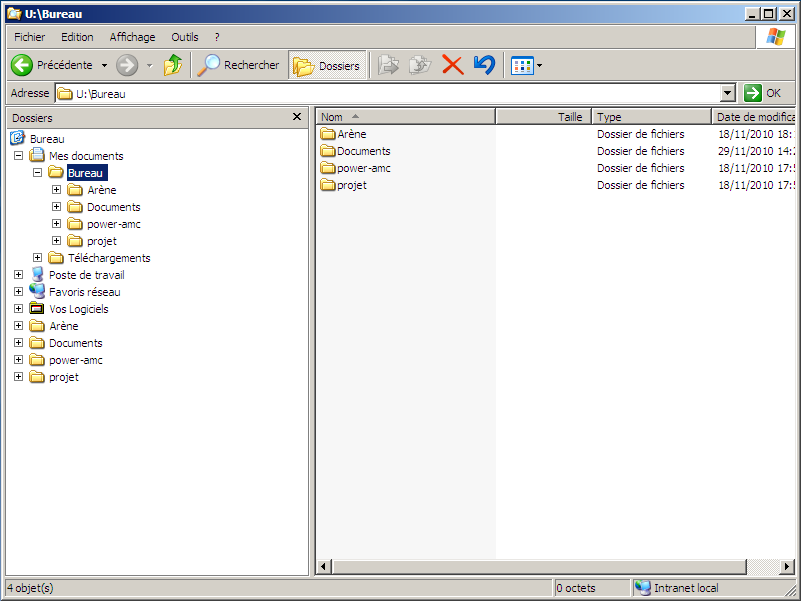
\includegraphics[height=2.5cm]{img/s02/explorer_windows.png}
        \end{center}
      \end{column}
      \begin{column}{6cm}
        \begin{center}
          Ligne de Commande\\
          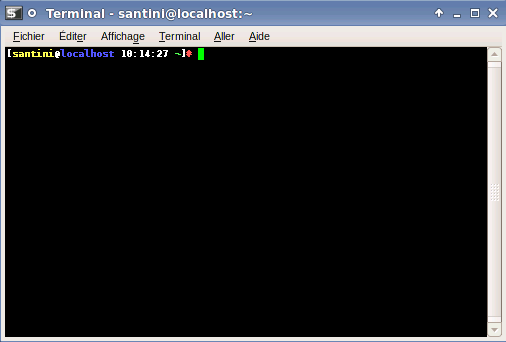
\includegraphics[height=2.5cm]{img/s02/terminal_single.png}
        \end{center}
      \end{column}
    \end{columns}
  \end{block}
  \begin{block}{Principales commandes}
    \begin{center}
      \begin{tabular}{ll}
        \hline
        Commande&Fonction principale\\
        \hline
        \lin{pwd}&Afficher le nom du répertoire courant\\
        \lin{ls}&Afficher le contenu d'un répertoire\\
        \lin{cd}&Changer de répertoire courant\\
        \lin{mkdir}&Créer un répertoire\\
        \lin{rm}&Supprimer fichier(s) ou répertoire(s) \\
        \lin{cp}&Copier fichier(s) ou répertoire(s)\\
        \lin{mv}&Déplacer/Renommer fichier(s) ou répertoire(s)\\
        \hline
      \end{tabular}
    \end{center}
  \end{block}
\end{frame}
\manpage{pwd} \manpage{ls} \manpage{ls(bis)} \manpage{cd}
\manpage{mkdir} \manpage{rm} \manpage{rm(bis)} \manpage{cp}
\manpage{cp(bis)} \manpage{cp(ter)} \manpage{mv} \manpage{mv(bis)}
\manpage{mv(ter)}
\begin{exercice}
  \begin{exercicelet}{Préparation}
    \begin{enumerate}
    \item À l'issue du premier TP un répertoire nommé
      \verb|Intro_Systeme| doit se trouver dans votre répertoire
      personnel. Donnez la commande permettant d'afficher le contenu de
      ce répertoire.
    \item Donnez la commande permettant d'afficher l'ensemble des
      fichiers contenus dans ce répertoire (y compris les fichiers
      cachés).
    \item Définissez la commande permettant de créer un répertoire pour
      le TP 2. Ce répertoire sera contenu dans le répertoire
      \verb|Intro_Systeme| et portera le nom \verb|TP_2|. Pour cela vous
      devrez d'abord définir le répertoire \verb|Intro_Systeme| comme
      votre répertoire courant.
    \item Téléchargez l'archive contenant les données pour le TP 2:
      Allez sur le site
      \url{http://www-lipn.univ-paris13.fr/~santini/documents_pedagogiques}.
      Téléchargez le fichier \verb|donnees_tdtp2.tar.gz|. Recherchez où
      le fichier a été écrit dans l'arborescence de votre répertoire
      personnel.
    \item Donnez la suite de commandes permettant de déplacer le fichier
      archive dans le répertoire \verb|TP_2| que vous venez de créer. À
      la fin des commandes, le répertoire \verb|TP_2| sera toujours
      votre répertoire courant.
    \item Quelle commande permet de vérifier que l'archive est bien dans
      le répertoire \verb|~/Intro_systeme/TP_2|?
      \setcounter{cnti}{\value{enumi}}
    \end{enumerate}
  \end{exercicelet}
\end{exercice}
\begin{exercice}
  \begin{exercicelet}{Préparation}
    \begin{enumerate}\setcounter{enumi}{\value{cnti}}
    \item Quelles sont les informations données par le nom du fichier?
    \item Les commandes \texttt{less} et \texttt{cat} permettent
      d'afficher le contenu d'un fichier. Analysez la différence de
      comportement entre ces deux commandes sur le fichier
      \verb|donnees_tdtp2.tar.gz|. Qu'en concluez-vous?
    \item La commande \verb|tar xvf fichier| permet de désarchiver une
      archive non compressée, \texttt{gunzip} de décompresser un fichier
      et \texttt{gzip} de le compresser. Sachant cela, quelle suite de
      commandes faut-il taper pour extaire les données de l'archive
      \verb|donnees_tdtp2.tar.gz|? Un répertoire était contenu dans
      l'archive. Quel est son nom?
    \item Les commandes \texttt{less} et \texttt{cat} permettent
      d'afficher le contenu d'un fichier. Analysez la différence de
      comportement entre ces deux commandes sur le fichier
      \verb|donnees/command_line.txt|. Qu'en concluez-vous?
      \setcounter{cnti}{\value{enumi}}
    \end{enumerate}
    
    Remarques: si un affichage prend trop de temps, utilisez le
    raccourci clavier adéquat pour suspendre l'exécution de la commande
    courante.  Si l'affichage de votre terminal est durablement
    perturbé, dans le menu Terminal \textrightarrow Réinitialiser le
    terminal.
  \end{exercicelet}
\end{exercice}
\subsection{Métacaractères}
\begin{frame}{Le métacaractère \lin{*}}
  \begin{block}{Le caractère \lin{*}}
    \begin{itemize}
    \item Le cataractère \lin{*} est utilisé comme un \textit{jocker}
      pour remplacer une chaîne de caractères,
    \item Il est utilisé pour pointer plusieurs fichiers ou répertoires
      dont le nom partage un motif commun.
    \item Le caractère \lin{*} peut être placé en début, en fin ou au
      milieu d'une chaîne de caractères,
    \item Le caractère \lin{*} peut être répété.
    \end{itemize}
  \end{block}
  \begin{block}{Exemple de manipulation avec la commande \lin{mv}}
    \scriptsize{
      \begin{columns}
        \begin{column}{6cm}
          \begin{center}
            \mpromptS{%
              \promptS{mv *.jpg Images/}{} }
          \end{center}
        \end{column}
        \begin{column}{6cm}
          Ici, le chemin \lin{*.jpg} pointe tous les fichiers du
          répertoire courant dont le nom se fini par l'extension
          \lin{.jpg}. Il pointe donc les fichiers \lin{etacentauri.jpg}
          et \lin{aldebaran.jpg} et exclue les autres fichiers (ici le
          fichier \lin{alphacentauri.gif}).
        \end{column}
      \end{columns}
      \begin{columns}
        \begin{column}{6cm}
          \dirtree{%
            .1
            \DTd{{\color{solarizedRed}chez\_moi}}\DTfcomment{{\color{solarizedRed}Répertoire
                Courant}}.  .2 aldebaran{\color{solarizedGreen}.jpg}
            \DTfcomment{{\color{solarizedGreen}Fichier ciblé}}.  .2
            alphacentauri.gif .  .2
            etacentauri{\color{solarizedGreen}.jpg}
            \DTfcomment{{\color{solarizedGreen}Fichier ciblé}}.  .2
            \DTd{{\color{solarizedBlue}Images}}\DTfcomment{{\color{solarizedBlue}Répertoire
                final}}.  }
        \end{column}
        \begin{column}{6cm}
          \dirtree{%
            .1
            \DTd{{\color{solarizedRed}chez\_moi}}\DTfcomment{{\color{solarizedRed}Répertoire
                Courant}}.  .2 alphacentauri.gif .  .2
            \DTd{{\color{solarizedBlue}Images}}\DTfcomment{{\color{solarizedBlue}Répertoire
                final}}.  .3 {\color{solarizedGreen}aldebaran.jpg}
            \DTfcomment{{\color{solarizedGreen}Fichier déplacé}}.  .3
            {\color{solarizedGreen} etacentauri.jpg}
            \DTfcomment{{\color{solarizedGreen}Fichier déplacé}}.  }
        \end{column}
      \end{columns}
    }
  \end{block}
\end{frame}
\begin{frame}{Exemples d'utilisation de l'étoile}
  \begin{block}{Utilisation simple avec la commande \lin{mv}}
    \scriptsize{
      \begin{columns}
        \begin{column}{6cm}
          \begin{center}
            \mpromptS{%
              \promptS{mv al* Images/}{} }
          \end{center}
        \end{column}
        \begin{column}{6cm}
          Ici, le chemin \lin{al*} pointe tous les fichiers du
          répertoire courant dont le nom commence par les caractères
          \lin{al}. Il pointe donc les fichiers \lin{aldebaran.jpg} et
          \lin{alphacentauri.gif} et exclue les autres fichiers (ici le
          fichier \lin{etacentauri.jpg}).
        \end{column}
      \end{columns}
      \begin{columns}
        \begin{column}{6cm}
          \dirtree{%
            .1
            \DTd{{\color{solarizedRed}chez\_moi}}\DTfcomment{{\color{solarizedRed}Répertoire
                Courant}}.  .2 {\color{solarizedGreen}al}debaran.jpg
            \DTfcomment{{\color{solarizedGreen}Fichier ciblé}}.  .2
            {\color{solarizedGreen}al}phacentauri.gif
            \DTfcomment{{\color{solarizedGreen}Fichier ciblé}}.  .2
            etacentauri.jpg.  .2
            \DTd{{\color{solarizedBlue}Images}}\DTfcomment{{\color{solarizedBlue}Répertoire
                final}}.  }
        \end{column}
        \begin{column}{6cm}
          \dirtree{%
            .1
            \DTd{{\color{solarizedRed}chez\_moi}}\DTfcomment{{\color{solarizedRed}Répertoire
                Courant}}.  .2 etacentauri.jpg .  .2
            \DTd{{\color{solarizedBlue}Images}}\DTfcomment{{\color{solarizedBlue}Répertoire
                final}}.  .3 {\color{solarizedGreen}aldebaran.jpg}
            \DTfcomment{{\color{solarizedGreen}Fichier déplacé}}.  .3
            {\color{solarizedGreen}alphacentauri.gif}
            \DTfcomment{{\color{solarizedGreen}Fichier déplacé}}.  }
        \end{column}
      \end{columns}
    }
  \end{block}
  \begin{block}{Utilisation double avec la commande \lin{mv}}
    \scriptsize{
      \begin{columns}
        \begin{column}{6cm}
          \begin{center}
            \mpromptS{%
              \promptS{mv *centauri* JPG/}{} }
          \end{center}
        \end{column}
        \begin{column}{6cm}
          Ici, le chemin \lin{*centauri*} pointe tous les fichiers du
          répertoire courant dont le nom contient la chaîne de
          caractères \lin{centauri}. Il pointe donc les fichiers
          \lin{alphacentauri.gif} et \lin{etacentauri.jpg} et exclue les
          autres fichiers (ici le fichier \lin{aldebaran.jpg}).
        \end{column}
      \end{columns}
      \begin{columns}
        \begin{column}{6cm}
          \dirtree{%
            .1
            \DTd{{\color{solarizedRed}chez\_moi}}\DTfcomment{{\color{solarizedRed}Répertoire
                Courant}}.  .2 aldebaran.jpg .  .2
            alpha{\color{solarizedGreen}centauri}.gif
            \DTfcomment{{\color{solarizedGreen}Fichier ciblé}}.  .2
            eta{\color{solarizedGreen}centauri}.jpg
            \DTfcomment{{\color{solarizedGreen}Fichier ciblé}}.  .2
            \DTd{{\color{solarizedBlue}Images}}\DTfcomment{{\color{solarizedBlue}Répertoire
                Final}}.  }
        \end{column}
        \begin{column}{6cm}
          \dirtree{%
            .1
            \DTd{{\color{solarizedRed}chez\_moi}}\DTfcomment{{\color{solarizedRed}Répertoire
                Courant}}.  .2 aldebaran.jpg .  .2
            \DTd{{\color{solarizedBlue}Images}}\DTfcomment{{\color{solarizedBlue}Répertoire
                final}}.  .3 {\color{solarizedGreen}alphacentauri.gif}
            \DTfcomment{{\color{solarizedGreen}Fichier déplacé}}.  .3
            {\color{solarizedGreen}etcentauri.jpg}
            \DTfcomment{{\color{solarizedGreen}Fichier déplacé}}.  }
        \end{column}
      \end{columns}
    }
  \end{block}
\end{frame}
\begin{frame}{Métacaractère et chemins ciblés}
  \begin{block}{Exemple plus complexe et Détails de l'interprétation}
    \begin{itemize}
    \item Le cararctère \lin{*} est développé lors de l'interprétation.
    \end{itemize}
  \end{block}
  \begin{center}
    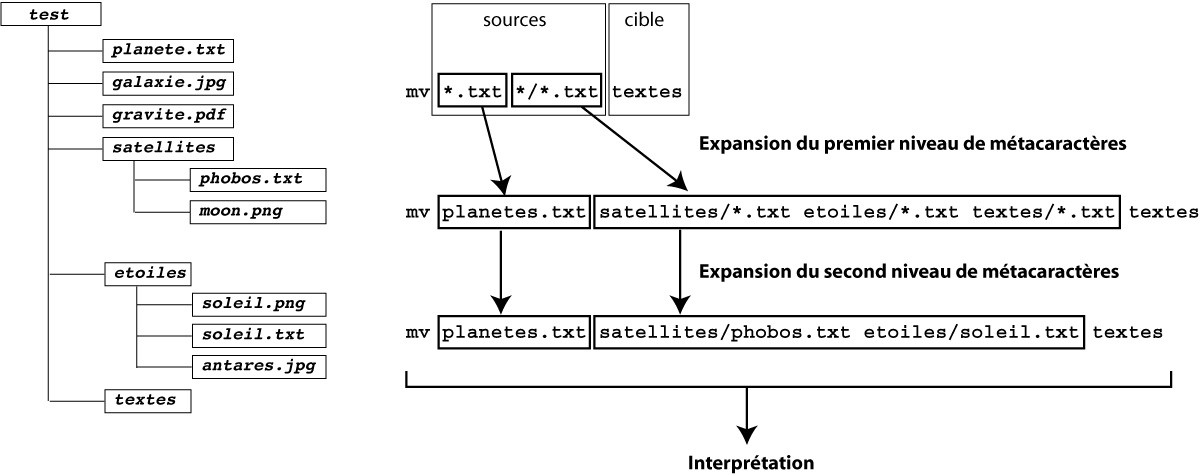
\includegraphics[width=12cm]{img/s02/star_met_mv_interp.jpg}
  \end{center}
\end{frame}
\begin{exercice}
  \begin{exercicelet}{Interprétation de l'étoile}
    \begin{enumerate}\setcounter{enumi}{\value{cnti}}
    \item Quelle commande permet la création d'un répertoire nommé
      \texttt{JPG}?
    \item Quelle commande permet la création "simultanée" de deux
      répertoires nommés \texttt{GIF} et \texttt{PNG}?
    \item Quelle commande permet de déplacer depuis le répertoire
      \texttt{images} tous les fichiers présentant l'extension
      \texttt{jpg} dans le répertoire \texttt{JPG} nouvellement créé?
    \item Quelle commande permet de copier depuis le répertoire
      \texttt{images} tous les fichiers présentant l'extension
      \texttt{png} dans le répertoire \texttt{PNG} nouvellement créé?
    \item Définissez le répertoire \texttt{GIF} comme votre répertoire
      courant. Quelle commande permet de déplacer les fichiers du
      répertoire \texttt{images} dont l'extension est \texttt{gif} dans
      le répertoire \texttt{GIF}?
    \item Quel est le résultat de la séquence de commandes suivante?:
\begin{verbatim}
 cd ..
 rm images
\end{verbatim}
    \item Comment modifier la dernière commande pour supprimer le
      répertoire \texttt{images/}? Comment modifier la commande pour
      éviter les invites de confirmation?
    \item Quelle commande permet de copier le répertoire \texttt{GIF} et
      son contenu dans un répertoire nommé \verb|images_GIF|?
    \item Quelle est la fifférence entre les deux commandes suivantes:
\begin{verbatim}
      cd ~
      cd /home/usager/votre_identifiant/
\end{verbatim}
    \item Donnez une commande utilisant le chemin absolu du répertoire
      \verb|Intro_systeme| permettant de réaliser un copie nommée
      \verb|Intro_Systeme_BackUp| de ce répertoire, dans votre
      répertoire personnel.  \setcounter{cnti}{\value{enumi}}
    \end{enumerate}
  \end{exercicelet}
\end{exercice}
